\documentclass[12pt]{article}
\usepackage{array}
\usepackage{amsmath}
\usepackage{amssymb}
\usepackage{mathtools}
\usepackage{textcomp}
\usepackage{gensymb}
\usepackage{graphicx}
\usepackage{float}
\usepackage{caption}
\usepackage{amsfonts}
\usepackage[margin=1in]{geometry}

\newcounter{results}
\newcounter{questions}

\def\neg{{\sim}}
\def\Z{\mathbb{Z}}
\def\N{\mathbb{N}}
\def\R{\mathbb{R}}
\def\Q{\mathbb{Q}}
\def\E{\mathbb{E}}
\def\qed{\(\blacksquare\)}
\newcommand{\result}[1]{\stepcounter{results}{\bfseries Result \arabic{results}}: #1}
\newcommand{\question}[1]{\stepcounter{questions}{\bf \arabic{questions}}: #1}
\newenvironment{proof}[2][Proof]{\result{#2}\begin{trivlist} 
    \item[\hskip \labelsep {\sc #1:}]}{\qed\end{trivlist}}

\begin{document}
    \title{Computational Assignment \#3}
    \author{Ryan Coyne}
    \maketitle
    \noindent \(T = 300\) K:\\
    Z = 0.0257000324254782\\
    Analytic Mean = 0.025699967574562714\\
    Numerical Mean = 0.025699935142720585\\
    Analytic Variance = 0.0006604899999989488\\
    Numerical Variance = 0.0006604916669912035\\
    \(T = 500\) K:\\
    Z :  0.0428333527886234\\
    Analytic Mean = 0.04283331387805211\\
    Numerical Mean = 0.042833294343230716\\
    Analytic Variance = 0.0018346944444440655\\
    Numerical Variance = 0.0018346960388592663\\
    \(T = 1000\) K:\\
    Z = 0.08566667639431236\\
    Analytic Mean = 0.08566665693902209\\
    Numerical Mean = 0.08565739786178304\\
    Analytic Variance = 0.007338777777777682\\
    Numerical Variance = 0.007330259849358138\\
    \begin{figure}[H]
        \centering
        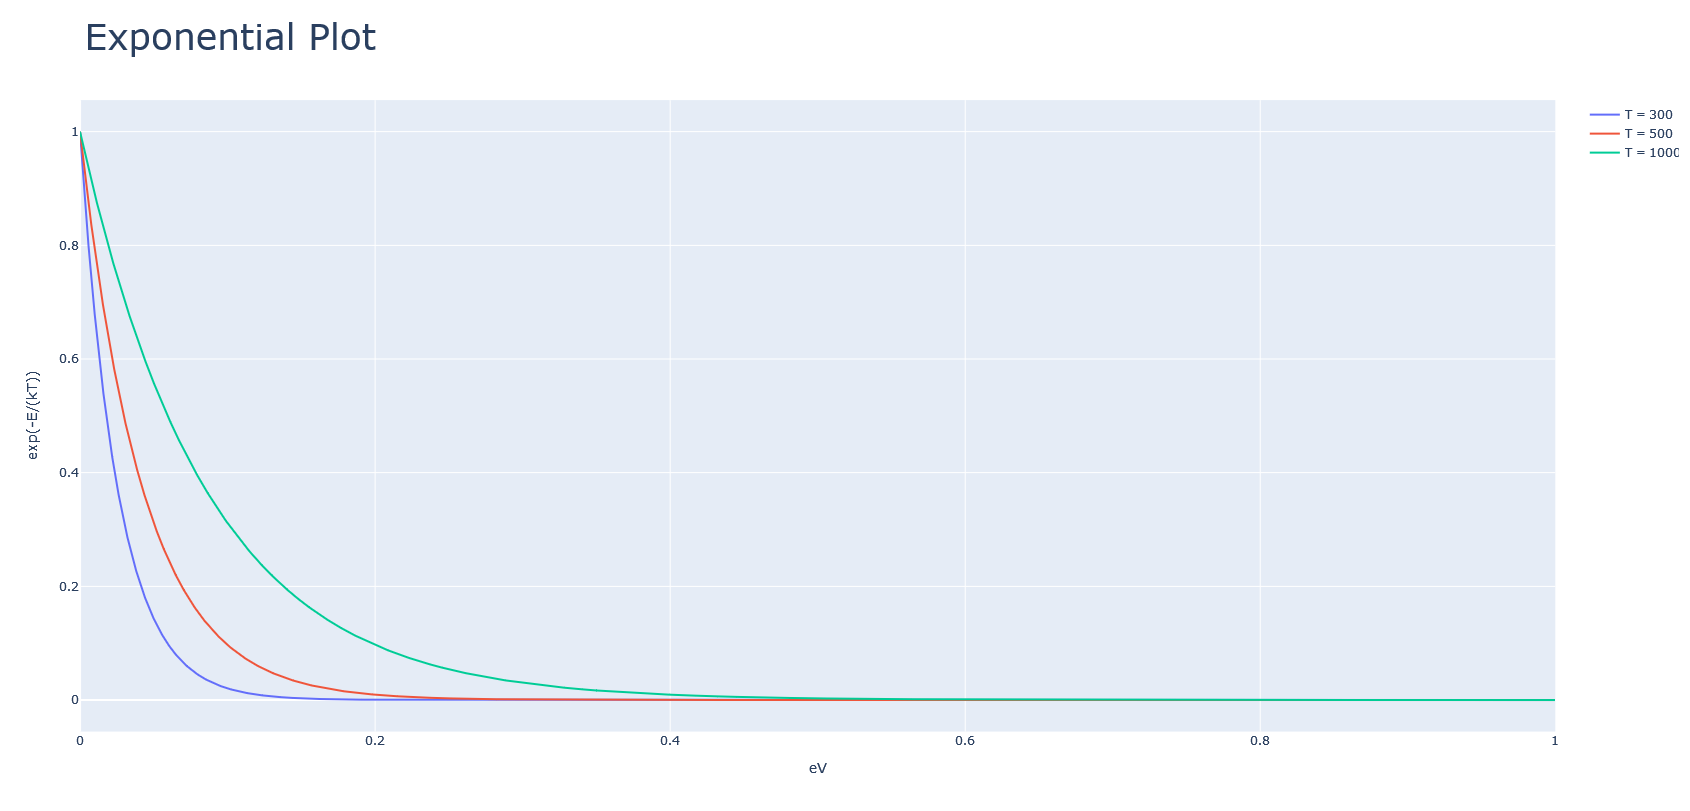
\includegraphics[width=\linewidth]{fig1.png}
    \end{figure}
    \begin{figure}
        \centering
        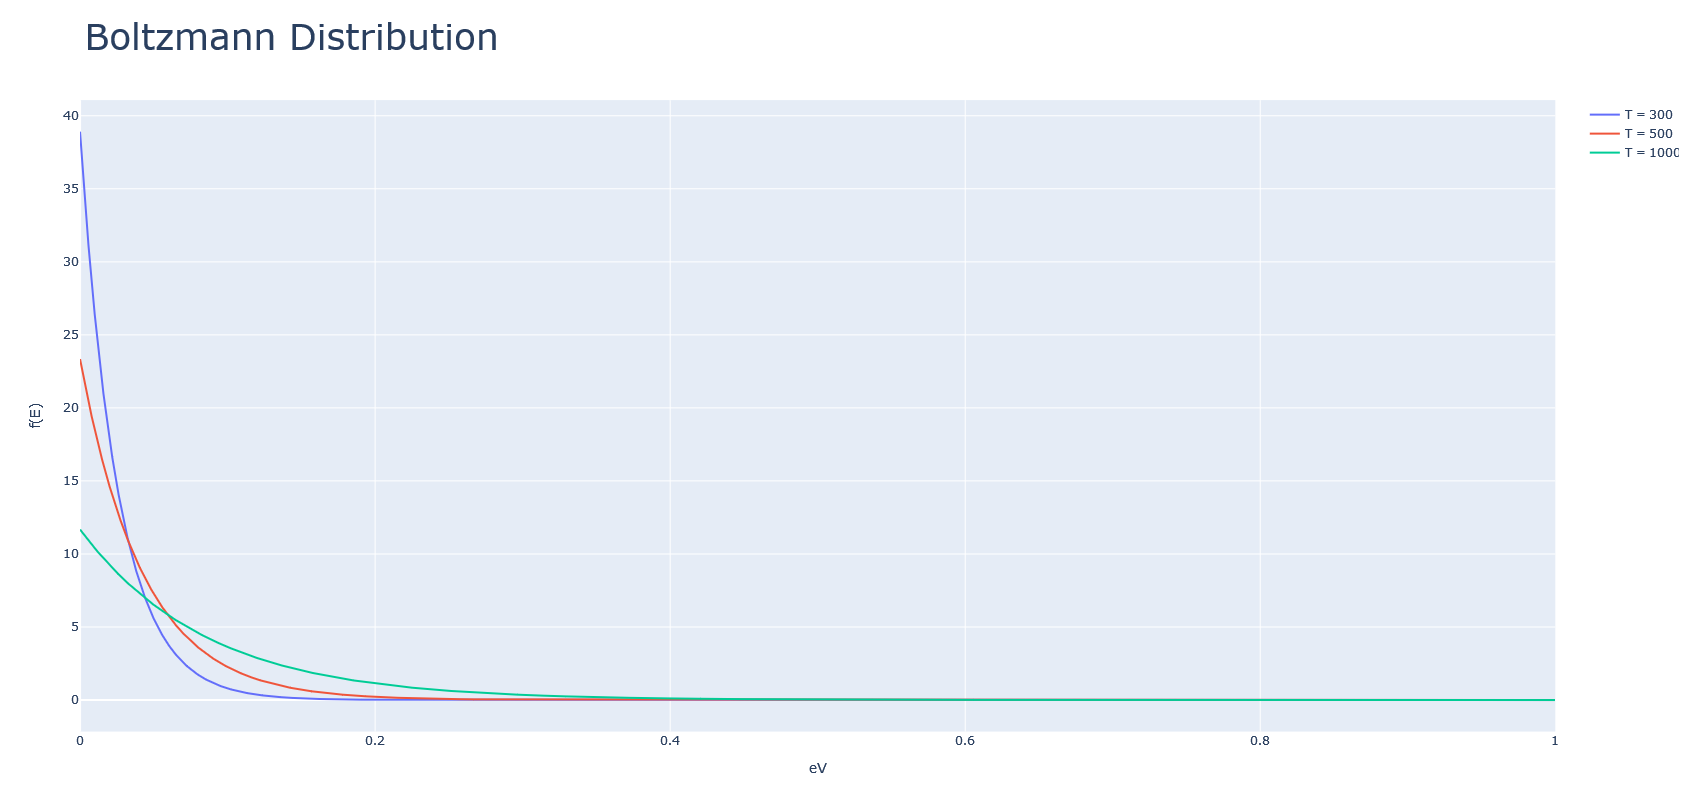
\includegraphics[width=\linewidth]{fig2.png}
    \end{figure}
    \begin{figure}
        \centering
        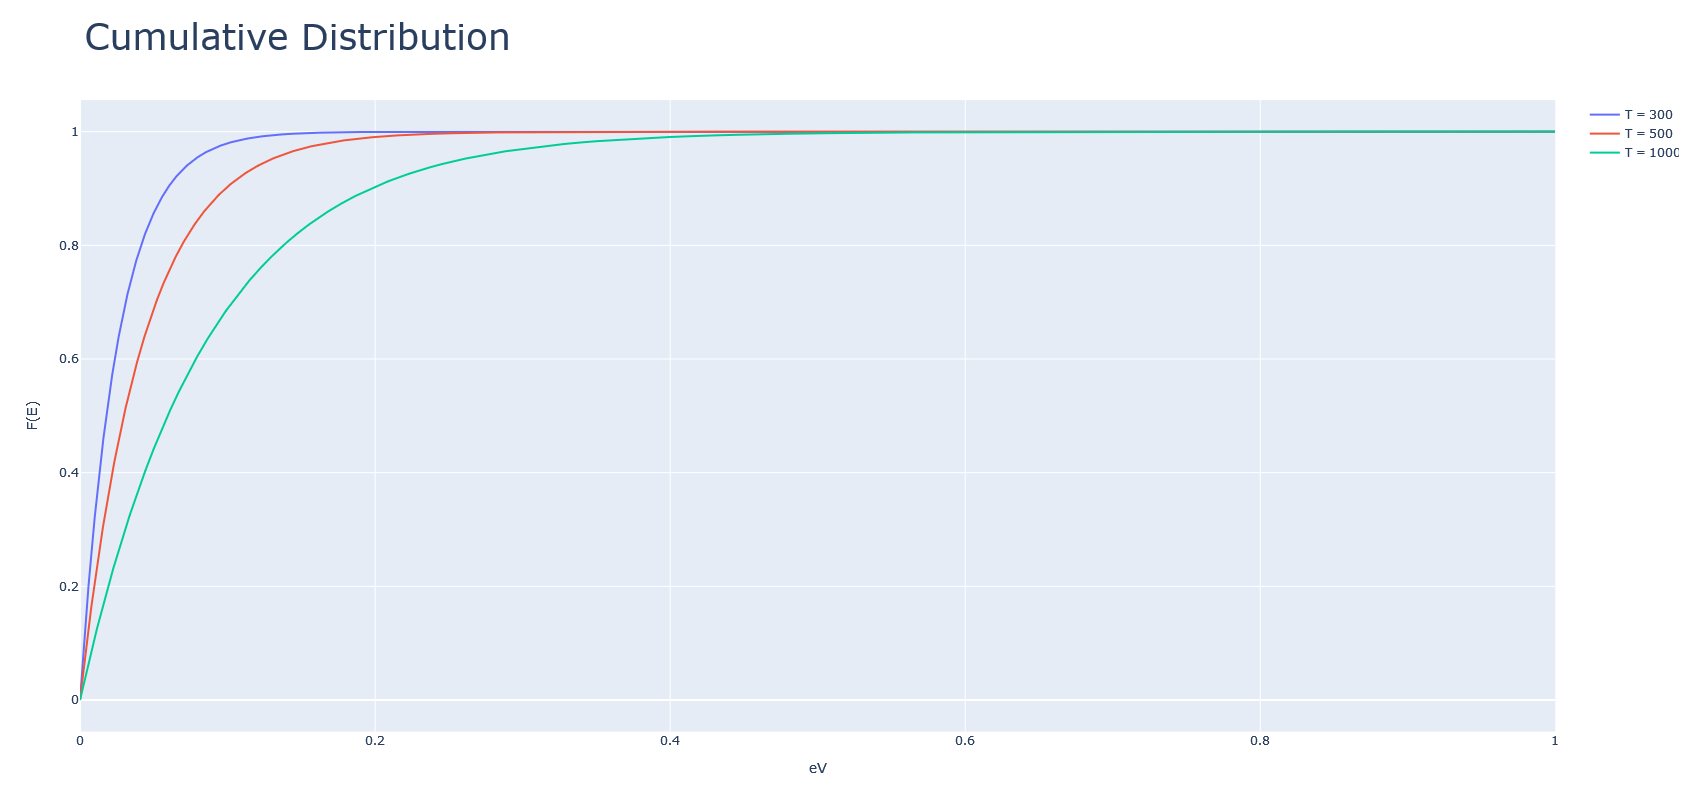
\includegraphics[width=\linewidth]{fig3.png}
    \end{figure}
\end{document}